% =====================================================================
% Section 4.6  Dynamic left ventricular problem
% Data: results_paper/gls_pdf_fs_h0.35 (run_paper_case.command: GLS P1/P1 on the
%       h = 0.35 cm mesh, mu_eff^HO of Eq. (43) incl. fs term, c_t = 1.5, c_s = 3.0,
%       C_tau = 0.03, C_c = 0.1), extracted by extract_data.py to
%       data/lv_timeseries.csv; plots by make_figures.py.
% ParaView: results_paper/gls_pdf_fs_h0.35/vtk/gls.pvd, frame k <-> t = 0.005 (k+1) s.
% Equation/figure numbers of earlier sections are hard-coded via \Eqref{..};
% replace by \eqref{<your label>} in the main document if preferred.
% Figures marked "ParaView" are placeholders: drop the PNG/PDF with the
% given file name into figures/ and it is picked up automatically.
% =====================================================================
\providecommand{\Eqref}[1]{Eq.~(#1)}
\providecommand{\lvfig}[3]{% #1 file (no ext) #2 width #3 placeholder text
  \IfFileExists{figures/#1.png}{\includegraphics[width=#2]{figures/#1.png}}{%
  \IfFileExists{figures/#1.pdf}{\includegraphics[width=#2]{figures/#1.pdf}}{%
  \fbox{\parbox[c][0.62#2][c]{0.9#2}{\centering\scriptsize\textsf{ParaView:}\\[2pt] #3\\[2pt]\texttt{\detokenize{#1}}}}}}}

\subsection{Dynamic left ventricular problem}
\label{sec:lv}

A dynamic left-ventricular (LV) problem is finally considered to assess the proposed
GLS-stabilized $P_1/P_1$ formulation in a cardiac-mechanics setting. Compared with the
preceding benchmarks, this problem combines a curved three-dimensional geometry, an
anisotropic exponential constitutive law with a spatially varying fiber architecture,
active fiber contraction, a follower pressure load, and mixed Robin and penalty-type
boundary conditions, all under strict incompressibility and strongly time-dependent
loading over a full cardiac cycle. The purpose of this example is to demonstrate that the
formulation, with the stabilization parameters of Section~3.3 kept unchanged, can follow
the large deformation of the ventricle through filling, contraction, and relaxation while
maintaining a stable pressure field.

\paragraph{Geometry, mesh, and fiber architecture.}
The LV is represented by an idealized truncated prolate ellipsoid with the long axis along
$X_1$ (Fig.~\ref{fig:lv_setup}). The endocardial and epicardial surfaces are ellipsoids
with semi-axes $(9.0,\,2.5,\,2.5)$\,cm and $(9.7,\,3.5,\,3.5)$\,cm, respectively, and the
base is a conical cut between $X_1=2.65$\,cm on the endocardium and $X_1=2.43$\,cm on the
epicardium. The reference cavity volume is $V_0=167.7$\,mL. The myocardium is discretized
with 21\,707 linear tetrahedra and 5840 vertices, i.e., 23\,360 velocity--pressure degrees
of freedom, with element sizes $h_K\in[2.6,\,8.2]$\,mm; the boundary consists of 3590
endocardial, 4638 epicardial, and 430 basal facets. The fiber field follows a rule-based
construction: a transmural coordinate $\phi\in[0,1]$ is obtained from a Laplace problem with
$\phi=0$ on the endocardium and $\phi=1$ on the epicardium, and the fiber direction
$\mathrm{f}_0$ is rotated in the local circumferential--longitudinal plane with a helix
angle varying linearly from $+60^\circ$ at the endocardium to $-60^\circ$ at the epicardium.
The sheet direction $\mathrm{s}_0$ is aligned with the transmural direction. Both fields are
sampled at the element centroids and re-orthonormalized, giving elementwise constant
$\mathrm{f}_0$ and $\mathrm{s}_0$ (Fig.~\ref{fig:lv_setup}b,c).

\begin{figure}[htbp]
  \centering
  \begin{subfigure}[b]{0.32\textwidth}\centering
    \lvfig{lv_geometry}{\linewidth}{reference geometry and mesh;\\ base / endo / epi facets colored}
    \caption{Geometry and mesh}
  \end{subfigure}\hfill
  \begin{subfigure}[b]{0.32\textwidth}\centering
    \lvfig{lv_fiber}{\linewidth}{fiber direction $\mathrm{f}_0$ (glyphs),\\ cut-away view}
    \caption{Fiber direction $\mathrm{f}_0$}
  \end{subfigure}\hfill
  \begin{subfigure}[b]{0.32\textwidth}\centering
    \lvfig{lv_sheet}{\linewidth}{sheet direction $\mathrm{s}_0$ (glyphs)}
    \caption{Sheet direction $\mathrm{s}_0$}
  \end{subfigure}
  \caption{Dynamic left ventricular problem: idealized geometry, finite element mesh with the
  basal, endocardial, and epicardial boundaries, and the rule-based fiber and sheet fields.}
  \label{fig:lv_setup}
\end{figure}

\paragraph{Constitutive model and active stress.}
The passive myocardium is described by the incompressible Holzapfel--Ogden model
\Eqref{19}, with the fiber and sheet invariants computed from $\mathbb{C}$ as in
\Eqref{7} and the positive parts regularized as in Section~3.3. The material parameters are
listed in Table~\ref{tab:lv_parameters}. A viscous contribution
$W_{\mathrm{vis}}=\tfrac{\eta}{2}\,\mathrm{tr}(\dot{\mathbb{E}}^2)$, with
$\dot{\mathbb{E}}=\mathbb{F}^T\mathbb{d}\,\mathbb{F}$ and
$\mathbb{d}=\mathrm{sym}(\dot{\mathbb{F}}\mathbb{F}^{-1})$, and an active fiber stress
\begin{equation}
  \mathbb{P}_{\mathrm{act}} = T_a(t)\left[1+4.9\left(\sqrt{\bar I_{4\mathrm{f}}}-1\right)\right]
  \mathbb{F}\,\mathrm{f}_0\otimes\mathrm{f}_0,
  \qquad \bar I_{4\mathrm{f}}=\mathrm{f}_0\cdot\bar{\mathbb{C}}\,\mathrm{f}_0,
  \label{eq:lv_active}
\end{equation}
are added to the deviatoric stress, so that the total first Piola--Kirchhoff stress reads
$\mathbb{P}_{\mathrm{dev}}+\mathbb{F}\,\eta\,\dot{\mathbb{E}}+\mathbb{P}_{\mathrm{act}}-p\,\mathbb{H}$.
These additional stresses enter both the Galerkin terms and the strong momentum residual
$\mathbf{R}_{m,h}$ in Eq.~(23); the GLS formulation itself is not modified. The effective
stiffness in the stabilization parameters is $\mu_{\mathrm{eff}}^{\mathrm{HO}}$ of
\Eqref{43}, including the fiber--sheet coupling term, and the coefficients are those used
for all anisotropic examples, $c_t=1.5$, $c_s=3.0$, $C_\tau=0.03$, and $C_c=0.1$.

\paragraph{Loading and boundary conditions.}
The cardiac cycle is driven by a prescribed endocardial pressure $p_{\mathrm{endo}}(t)$ and
a prescribed active tension $T_a(t)$ (Fig.~\ref{fig:lv_loading}), in kPa and with $t$ in s,
\begin{align}
  p_{\mathrm{endo}}(t)&=
  \begin{cases}
    1.067\,t/0.2, & 0\le t<0.2,\\
    1.067, & 0.2\le t<0.5 \ \text{or}\ t\ge 0.8,\\
    1.067+13.46\left[1-e^{-(t-0.5)^2/0.004}\right], & 0.5\le t<0.65,\\
    1.067+13.46\left[1-e^{-(0.8-t)^2/0.004}\right], & 0.65\le t<0.8,
  \end{cases}
  \label{eq:lv_loading}\\
  T_a(t)&=
  \begin{cases}
    0, & t<0.5 \ \text{or}\ t\ge 0.8,\\
    84.26\left[1-e^{-(t-0.5)^2/0.005}\right], & 0.5\le t<0.65,\\
    84.26\left[1-e^{-(0.8-t)^2/0.005}\right], & 0.65\le t<0.8.
  \end{cases}
  \label{eq:lv_active_tension}
\end{align}
The ventricle is thus passively filled to an end-diastolic pressure of 1.067\,kPa
(8\,mmHg), after which active contraction raises the cavity pressure to 14.5\,kPa
(109\,mmHg) at $t=0.65$\,s before relaxation returns the system to the diastolic state.
The boundary conditions are
\begin{align}
  \big(\mathbb{P}\,\mathbf{N}\big)\big|_{\Gamma_{\mathrm{endo}}} &= -p_{\mathrm{endo}}(t)\,\mathbb{H}\mathbf{N},
  \label{eq:lv_bc_endo}\\
  \big(\mathbb{P}\,\mathbf{N}\big)\big|_{\Gamma_{\mathrm{epi}}} &= -\beta_{\mathrm{epi}}\,(\mathbf{v}\cdot\mathbf{N})\,\mathbf{N},
  \label{eq:lv_bc_epi}\\
  \big(\mathbb{P}\,\mathbf{N}\big)\big|_{\Gamma_{\mathrm{base}}} &= -\gamma\left[(\mathbf{u}\cdot\mathbf{e}_1)\,\mathbf{e}_1
  + \left(\mathbb{I}_\perp-\hat{\mathbf{R}}\otimes\hat{\mathbf{R}}\right)\mathbf{r}\right],
  \label{eq:lv_bc_base}
\end{align}
where $\mathbb{P}$ denotes the total stress. Eq.~\eqref{eq:lv_bc_endo} is a follower
pressure load acting on the current endocardial surface, and Eq.~\eqref{eq:lv_bc_epi}
represents the damping of the surrounding tissue through a Robin-type condition on the
normal velocity. In Eq.~\eqref{eq:lv_bc_base}, $\mathbf{e}_1$ is the long-axis direction,
$\mathbb{I}_\perp=\mathbb{I}-\mathbf{e}_1\otimes\mathbf{e}_1$, $\mathbf{r}$ is the in-plane
position of a basal point relative to the base centre in the current configuration, and
$\hat{\mathbf{R}}$ is the corresponding unit radial direction in the reference configuration.
The basal penalty therefore suppresses longitudinal motion and circumferential rotation of
the base while allowing it to expand and contract radially, which removes the rigid-body
modes without clamping the base. All three conditions are natural boundary conditions of the
velocity--pressure formulation, and no Dirichlet condition is imposed on the velocity. The
system starts from rest in the stress-free reference configuration,
$\mathbf{u}_0=\mathbf{v}_0=\mathbf{0}$.

The cycle $t\in[0,1]$\,s is integrated with $\Delta t=5\times10^{-3}$\,s (200 steps), using
backward Euler for the first step and BDF2 thereafter (Section~3.2). Each step is solved by
Newton's method with a backtracking line search, absolute and relative residual tolerances
$10^{-10}$ and $10^{-9}$, and the MUMPS direct solver. The LV computations were performed
with DOLFINx~0.11 and PETSc~3.25; the complete residual, including the stabilization
parameters and their dependence on $\mathbb{F}$ through $\mu_{\mathrm{eff}}$, is linearized by
automatic differentiation.

\begin{table}[htbp]
  \centering
  \caption{Dynamic left ventricular problem: model and discretization parameters.}
  \label{tab:lv_parameters}
  \small
  \begin{tabular}{lll}
    \toprule
    Group & Parameter & Value \\
    \midrule
    Holzapfel--Ogden & $a,\ b$ & $224.49$\,Pa, $1.6215$ \\
                     & $a_{\mathrm f},\ b_{\mathrm f}$ & $2426.7$\,Pa, $1.8268$ \\
                     & $a_{\mathrm s},\ b_{\mathrm s}$ & $556.24$\,Pa, $0.7746$ \\
                     & $a_{\mathrm{fs}},\ b_{\mathrm{fs}}$ & $390.52$\,Pa, $1.695$ \\
    Viscosity, density & $\eta,\ \rho_0$ & $100$\,Pa\,s, $1000$\,kg/m$^3$ \\
    Boundary conditions & $\beta_{\mathrm{epi}},\ \gamma$ & $5\times10^{3}$\,Pa\,s/m, $10^{6}$\,Pa/m \\
    Fiber architecture & helix angle (endo $\to$ epi) & $+60^\circ \to -60^\circ$ \\
    GLS parameters & $c_t,\ c_s,\ C_\tau,\ C_c$ & $1.5,\ 3.0,\ 0.03,\ 0.1$ \\
    Discretization & elements / vertices / DOFs & 21\,707 / 5840 / 23\,360 \\
                   & $\Delta t$, steps & $5\times10^{-3}$\,s, 200 \\
    \bottomrule
  \end{tabular}
\end{table}

\begin{figure}[htbp]
  \centering
  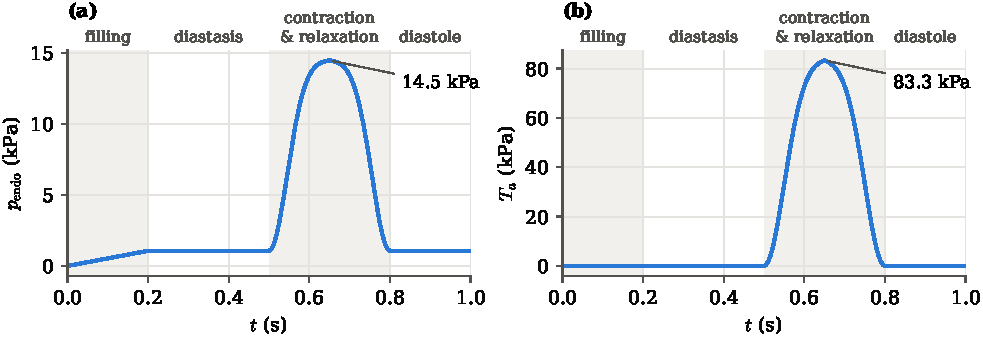
\includegraphics[width=0.92\textwidth]{figures/lv_loading.pdf}
  \caption{Dynamic left ventricular problem: prescribed (a) endocardial pressure and
  (b) active tension over one cardiac cycle, Eqs.~\eqref{eq:lv_loading}--\eqref{eq:lv_active_tension}. Shaded bands mark
  passive filling and the active phase.}
  \label{fig:lv_loading}
\end{figure}

\paragraph{Results.}
The simulation completes the full cycle without any adjustment of the time step or of the
stabilization parameters. Of the 200 steps, 195 converge in two or three Newton iterations
(Fig.~\ref{fig:lv_numerics}a); at most six iterations are needed at the onset of active
contraction ($t=0.52$--$0.54$\,s), where $T_a$ and $p_{\mathrm{endo}}$ rise most rapidly.
The largest final residual norm over the cycle is $2.5\times10^{-10}$.

Fig.~\ref{fig:lv_deformation} shows the deformed configurations at the reference state, at
end diastole ($t=0.5$\,s), at end systole ($t=0.655$\,s, minimum cavity volume), and at the
end of the cycle. The deformation is large throughout. During passive filling the cavity
volume increases from 167.7\,mL to 394.9\,mL, the long-axis length increases by 27\,\%
(from 122.3\,mm to 155.1\,mm), and the maximum displacement reaches 34.5\,mm, about
28\,\% of the reference long-axis length. Active contraction then reduces the cavity volume
to 145.7\,mL, corresponding to an ejection fraction of 63.1\,\%
(Fig.~\ref{fig:lv_global}a). The contraction exhibits the characteristic kinematics of the
ventricle: relative to end diastole, the long axis shortens by 11.6\,\% and the equatorial
wall thickens by 62\,\% (from 6.3\,mm to 10.2\,mm, Fig.~\ref{fig:lv_global}c). The
pressure--volume loop in Fig.~\ref{fig:lv_global}b displays the filling, contraction,
ejection, and relaxation phases of the cycle.

% CHECK with the ParaView pressure figure before submission: no checkerboard pattern at ED/ES/0.8 s.
Fig.~\ref{fig:lv_pressure} presents the pressure field $p_h$ on the deformed configurations.
The pressure remains smooth across the wall at all stages of the cycle, without the
element-scale checkerboard patterns of the unstabilized equal-order discretization observed
in the preceding benchmarks. Its extreme values stay bounded and follow the applied
cavity pressure (Fig.~\ref{fig:lv_numerics}c), with $p_h\in[-2.07,\,8.17]$\,kPa over the
cycle compared with the peak endocardial pressure of 14.5\,kPa. Since the incompressibility
constraint is imposed in the rate form of Eq.~(20c), the volume of the myocardial wall is
preserved in an integral sense: the mean Jacobian
$\bar J=|\Omega_0|^{-1}\int_{\Omega_0}J_h\,\mathrm{d}\Omega$ deviates from unity by at most
$0.20\,\%$ over the cycle (Fig.~\ref{fig:lv_numerics}b), and the deviation arises almost
entirely during the active phase.

These results show that the proposed GLS-stabilized $P_1/P_1$ formulation, with the
effective stiffness $\mu_{\mathrm{eff}}^{\mathrm{HO}}$ as the only model-dependent
ingredient of the stabilization parameters, carries over directly to an anisotropic,
actively contracting left ventricle with follower, Robin, and penalty-type boundary
conditions. It robustly captures the large global deformation through a complete cardiac
cycle while maintaining a stable pressure field.

\begin{figure}[htbp]
  \centering
  \begin{subfigure}[b]{0.24\textwidth}\centering
    \lvfig{lv_deformed_t0000}{\linewidth}{reference, $t=0$}
    \caption{$t=0$}
  \end{subfigure}\hfill
  \begin{subfigure}[b]{0.24\textwidth}\centering
    \lvfig{lv_deformed_t0500}{\linewidth}{end diastole, $t=0.5$\,s\\ (frame 99), $|\mathbf{u}_h|$}
    \caption{$t=0.5$\,s (ED)}
  \end{subfigure}\hfill
  \begin{subfigure}[b]{0.24\textwidth}\centering
    \lvfig{lv_deformed_t0655}{\linewidth}{end systole, $t=0.655$\,s\\ (frame 130), $|\mathbf{u}_h|$}
    \caption{$t=0.655$\,s (ES)}
  \end{subfigure}\hfill
  \begin{subfigure}[b]{0.24\textwidth}\centering
    \lvfig{lv_deformed_t1000}{\linewidth}{end of cycle, $t=1.0$\,s\\ (frame 199), $|\mathbf{u}_h|$}
    \caption{$t=1.0$\,s}
  \end{subfigure}
  \caption{Dynamic left ventricular problem: deformed configurations colored by the
  displacement magnitude $|\mathbf{u}_h|$ at the reference state, end diastole, end systole,
  and the end of the cycle. The gray outline indicates the reference configuration.}
  \label{fig:lv_deformation}
\end{figure}

\begin{figure}[htbp]
  \centering
  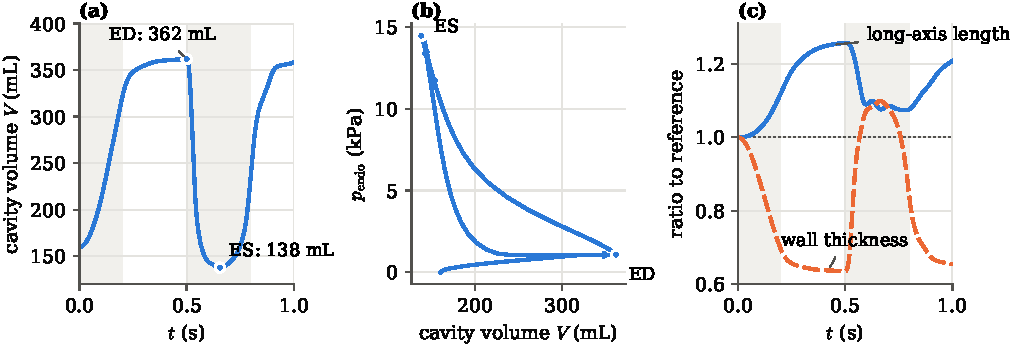
\includegraphics[width=\textwidth]{figures/lv_global_response.pdf}
  \caption{Dynamic left ventricular problem: global response. (a) Cavity volume, with end
  diastole (ED) and end systole (ES) marked; (b) pressure--volume loop; (c) long-axis length
  and equatorial wall thickness relative to the reference configuration. The cavity volume
  is computed exactly from the discrete endocardial surface as
  $V=-\frac{1}{3}\int_{\Gamma_{\mathrm{endo}}}(\mathbf{x}-\mathbf{x}_0)\cdot\mathbf{n}\,\mathrm{d}a$,
  with $\mathbf{x}_0$ on the basal plane of the endocardium.}
  \label{fig:lv_global}
\end{figure}

\begin{figure}[htbp]
  \centering
  \begin{subfigure}[b]{0.32\textwidth}\centering
    \lvfig{lv_pressure_t0500}{\linewidth}{$p_h$ at $t=0.5$\,s (ED),\\ long-axis cut}
    \caption{$t=0.5$\,s (ED)}
  \end{subfigure}\hfill
  \begin{subfigure}[b]{0.32\textwidth}\centering
    \lvfig{lv_pressure_t0655}{\linewidth}{$p_h$ at $t=0.655$\,s (ES),\\ long-axis cut}
    \caption{$t=0.655$\,s (ES)}
  \end{subfigure}\hfill
  \begin{subfigure}[b]{0.32\textwidth}\centering
    \lvfig{lv_pressure_t0800}{\linewidth}{$p_h$ at $t=0.8$\,s (end of relaxation),\\ long-axis cut}
    \caption{$t=0.8$\,s}
  \end{subfigure}
  \caption{Dynamic left ventricular problem: pressure field $p_h$ on the deformed
  configuration at end diastole, end systole, and the end of relaxation, shown on a
  long-axis cut through the wall.}
  \label{fig:lv_pressure}
\end{figure}

\begin{figure}[htbp]
  \centering
  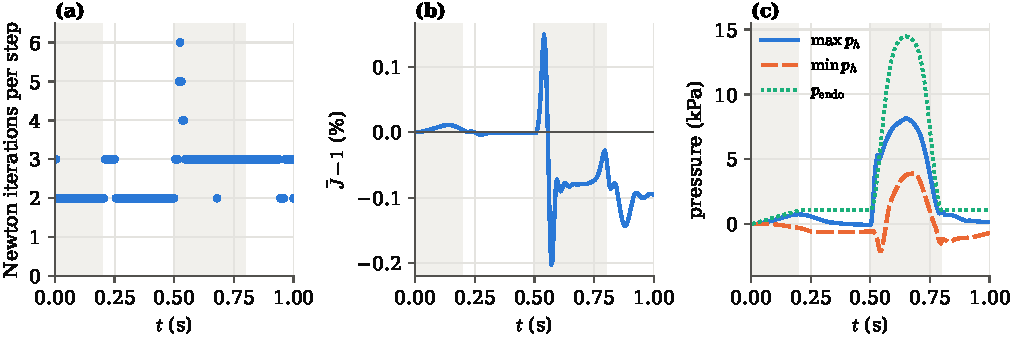
\includegraphics[width=\textwidth]{figures/lv_numerics.pdf}
  \caption{Dynamic left ventricular problem: (a) Newton iterations per time step; (b)
  deviation of the mean Jacobian $\bar J$ from unity; (c) extreme values of the pressure
  field compared with the prescribed endocardial pressure.}
  \label{fig:lv_numerics}
\end{figure}
